\chapter{Determinants}

\oldsection{Motivation}
By default, we can draw a coordinate plane over $\R^2$ by letting our elementary basis vectors $(1,0)$ and $(0,1)$ form grid lines. Notice that each of the squares in this grid has area $1$.
\begin{figure}[H]
\centering
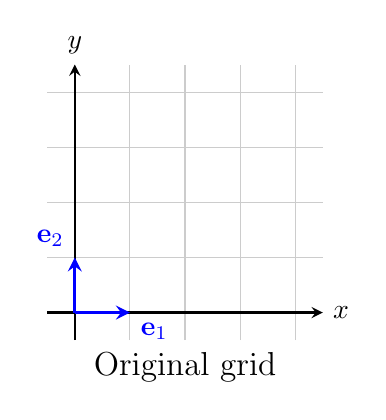
\begin{tikzpicture}[scale=0.7, >=stealth]
    % Draw grid
    \draw[step=1cm,gray!40,thin] (-0.5,-0.5) grid (4.5,4.5);

    % Axes
    \draw[->,thick] (-0.5,0) -- (4.5,0) node[right] {$x$};
    \draw[->,thick] (0,-0.5) -- (0,4.5) node[above] {$y$};

    % Basis vectors
    \draw[->,very thick,blue] (0,0) -- (1,0) node[below right] {$\mathbf{e}_1$};
    \draw[->,very thick,blue] (0,0) -- (0,1) node[above left] {$\mathbf{e}_2$};

    % Label
    \node at (2, -1) {\large Original grid};
\end{tikzpicture}
\caption{The standard basis and unit grid in $\mathbb{R}^2$.}
\end{figure}
Now consider a linear transformation on the standard basis by the matrix $A=\begin{bmatrix}
    2 & 1 \\
    0 & 2
\end{bmatrix}$. We can see in the figure below what it does to elementary basis and how this shifts the grid lines. Now our squares in the grid are larger. With a little bit of geometry, you can see that the new area of each square is $4$.
\begin{figure}[H]
\centering
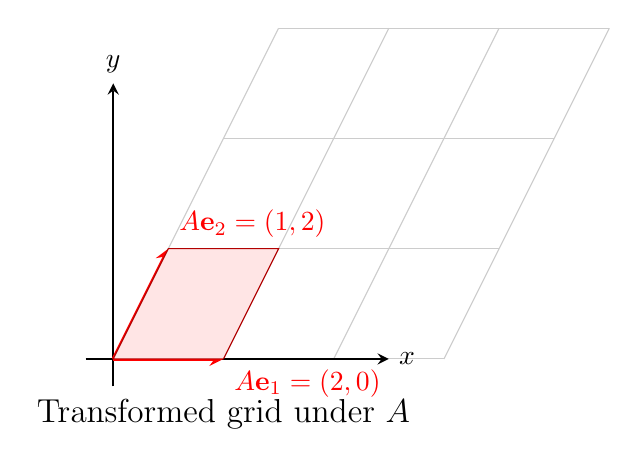
\begin{tikzpicture}[scale=0.7, >=stealth]
    % Transformation matrix vectors
    \def\a{2} % First column x
    \def\b{0} % First column y
    \def\c{1} % Second column x
    \def\d{2} % Second column y

    % Draw transformed grid
    \foreach \i in {0,...,3}{
        \draw[gray!40,thin] 
            ({\i*\a/1 + 0*\c}, {\i*\b/1 + 0*\d}) -- ({\i*\a/1 + 3*\c}, {\i*\b/1 + 3*\d});
        \draw[gray!40,thin]
            ({0*\a + \i*\c}, {0*\b + \i*\d}) -- ({3*\a + \i*\c}, {3*\b + \i*\d});
    }

    % Axes
    \draw[->,thick] (-0.5,0) -- (5,0) node[right] {$x$};
    \draw[->,thick] (0,-0.5) -- (0,5) node[above] {$y$};

    % Transformed basis vectors
    \draw[->,very thick,red] (0,0) -- (\a,\b) node[below right] {$A\mathbf{e}_1 = (2,0)$};
    \draw[->,very thick,red] (0,0) -- (\c,\d) node[above right] {$A\mathbf{e}_2 = (1,2)$};

    % Parallelogram showing the new unit cell
    \filldraw[fill=red!10, draw=red!70!black] 
      (0,0) -- (\a,\b) -- ({\a+\c},{\b+\d}) -- (\c,\d) -- cycle;

    % Label
    \node at (2, -1) {\large Transformed grid under $A$};
\end{tikzpicture}
\caption{The grid transformed by $A = \begin{bmatrix}2 & 1\\ 0 & 2\end{bmatrix}$.}
\end{figure}
The determinant of a linear transformation/matrix is a constant that is intended to capture this exact idea of area dilation. So for the example above, we would want the determinant of $A$ to be $4$ since the area grows four times. For this section, we will first talk about what properties we need the determinant to have in order to properly capture this dilation of area and then construct the determinant itself. We will see that if we define the properties in a certain way, the determinant is actually unique.
\begin{remark}
    The notion of "area" sort of breaks down if we are in arbitrary vector spaces/fields for example $\mathbb{P}^n$. However, everything we will discuss in this chapter will still hold. It is just much harder to interpret in arbitrary vector spaces/fields.
\end{remark}
\section{Desired Properties}
Let's begin discussing the desired properties. We will denote the determinant of a matrix $A$ as $\det(A)$. First of all, this notion of changing area only makes sense if we stay in the same dimension. If I transform from a square in $\R^2$ to a parallelepiped in $\R^3$, I'm changing from area to volume which is a huge distinction. How would you describe a change from area $4$ to volume $16$ in terms of a singular constant? You can't or at the very least people don't seem to have figured out how. Because of this, we only define the determinant for square matrices in which the transformation does not change dimension.
\begin{remark}
    I will be using the term "area" a lot, but you can interchange it with "volume" for higher dimension and everything will still hold.
\end{remark}
If we want a notion of changing area, we need a baseline for what area is. A simple way to do this is to look at the unit square/cube in $n$ dimensions. This always has area $1$ so it is a good baseline. Moreover, we can represent the unit cube using the identity matrix.
\begin{definition}
    Let $n\in\N$. We define $\det(I_n)=1$. This is known as the \textit{normalization} of the determinant.
\end{definition}
Now let's analyze what happens to the area under operations like vector addition and scalar multiplication. We'll again begin with the matrix $A_1=\begin{bmatrix}
    2 & 1 \\ 0 & 2
\end{bmatrix}$, but now we will compare it to the matrix $A_2=\begin{bmatrix}
    3 & 1 \\ 1 & 2
\end{bmatrix}$. This matrix results from adding $\begin{pmatrix}
    1 \\ 1
\end{pmatrix}$ to the transformation of $\vec{e}_1$.
\usetikzlibrary{calc}

\begin{figure}[H]
\centering
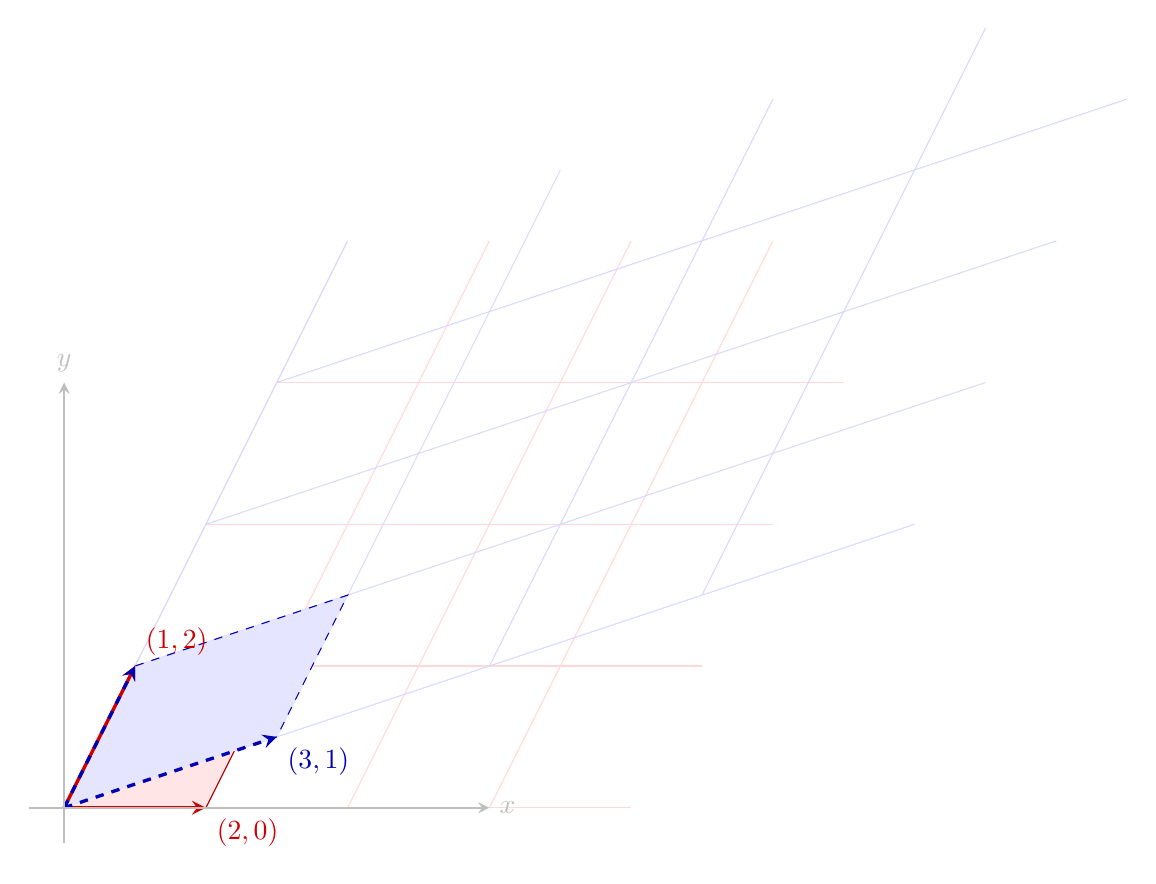
\begin{tikzpicture}[scale=0.9, >=stealth]

    % ====== Define columns for A1 ======
    \def\aOne{2} % first vector of A1
    \def\bOne{0}
    \def\cOne{1} % second vector of A1
    \def\dOne{2}

    % ====== Define columns for A2 ======
    \def\aTwo{3}
    \def\bTwo{1}
    \def\cTwo{1}
    \def\dTwo{2}

    % ===== Original Grid (A1) =====
    \foreach \i in {0,1,2,3} {
        % Lines parallel to v1 (shifted by multiples of v2)
        \draw[red!15, thin] ({\i*\cOne},{\i*\dOne}) -- ({\i*\cOne + 4*\aOne},{\i*\dOne + 4*\bOne});
    }
    \foreach \j in {0,1,2,3} {
        % Lines parallel to v2 (shifted by multiples of v1)
        \draw[red!15, thin] ({\j*\aOne},{\j*\bOne}) -- ({\j*\aOne + 4*\cOne},{\j*\bOne + 4*\dOne});
    }

    % ===== New Grid (A2) =====
    \foreach \i in {0,1,2,3} {
        \draw[blue!15, thin] ({\i*\cTwo},{\i*\dTwo}) -- ({\i*\cTwo + 4*\aTwo},{\i*\dTwo + 4*\bTwo});
    }
    \foreach \j in {0,1,2,3} {
        \draw[blue!15, thin] ({\j*\aTwo},{\j*\bTwo}) -- ({\j*\aTwo + 4*\cTwo},{\j*\bTwo + 4*\dTwo});
    }

    % ===== Parallelograms =====
    \filldraw[fill=red!10, draw=red!70!black]
        (0,0) -- (\aOne,\bOne) -- ({\aOne+\cOne},{\bOne+\dOne}) -- (\cOne,\dOne) -- cycle;
    \filldraw[fill=blue!10, draw=blue!70!black, dashed]
        (0,0) -- (\aTwo,\bTwo) -- ({\aTwo+\cTwo},{\bTwo+\dTwo}) -- (\cTwo,\dTwo) -- cycle;

    % ===== Vectors =====
    \draw[->,very thick,red!80!black] (0,0) -- (\aOne,\bOne) node[below right] {$(2,0)$};
    \draw[->,very thick,red!80!black] (0,0) -- (\cOne,\dOne) node[above right] {$(1,2)$};
    \draw[->,very thick,blue!70!black,dashed] (0,0) -- (\aTwo,\bTwo) node[below right] {$(3,1)$};
    \draw[->,very thick,blue!70!black,dashed] (0,0) -- (\cTwo,\dTwo);

    % ===== Axes (optional) =====
    \draw[->,thick,gray!50] (-0.5,0) -- (6,0) node[right] {$x$};
    \draw[->,thick,gray!50] (0,-0.5) -- (0,6) node[above] {$y$};

\end{tikzpicture}
\caption{Comparing the new transformation}
\end{figure}

\begin{definition}
    Let $V$ be a vector space over a field $\mathbb{F}$. Let $A$ be an $n\times n$ matrix where $A=[\vec{a}_1,\vec{a}_2,\dots,\vec{a}_n]$ where $\vec{a}_i$ is the $i$th column of $A$. For any arbitrary $\vec{v}\in V$ and $\alpha\in\mathbb{F}$, we define $\det([\vec{a}_1,\dots\alpha\vec{a}_i+\vec{v},\dots,\vec{a}_n])=\alpha\det([\vec{a}_1,\dots,\vec{a}_{i-1},\vec{a}_i,\dots,\vec{a}_n])+\det([\vec{a}_1,\dots,\vec{a}_{i-1},\vec{v},\dots,\vec{a}_n])$. This is known as the \textit{multi-linearity} property.
\end{definition}
One can do all the geometry and check that this property does in fact hold for the above transformation. However, it is much more useful to think about it broadly. If I scale one of the vectors, my area clearly increases by the scalar. If I add to one of my vectors, I am adding a new parallelogram to my current one which results in us adding the determinants.

Now let's look at another simple property. We have been analyzing what happens to the grid squares formed by the basis vectors, but what happens when the vectors are not linearly independent? For example, what if my transformation is $A=\begin{bmatrix}
    1 & 0 \\ 1 & 0
\end{bmatrix}$? This transformation maps $(1,0)$ and $(0,1)$ to $(1,0)$.
\begin{figure}[H]
\centering
\begin{tikzpicture}[scale=0.9, >=stealth]

    % Axes
    \draw[->,thick] (-0.5,0) -- (3,0) node[right] {$x$};
    \draw[->,thick] (0,-0.5) -- (0,2) node[above] {$y$};

    % Basis vectors (both same)
    \draw[->,very thick,red] (0,0) -- (1,0) node[below right] {$(1,0)$};
    \draw[->,very thick,red] (0,0) -- (1,0);

    % Degenerate "parallelogram"
    \filldraw[fill=red!10, draw=red!70!black, dashed]
      (0,0) -- (1,0) -- (2,0) -- (1,0) -- cycle;
\end{tikzpicture}
\caption{When both vectors are identical, the parallelogram collapses into a line, and the area is zero.}
\end{figure}

So in this case, we want the determinant to be $0$. Briefly, let's talk about what this means in higher dimensions. If I have two vectors that are the same, I've essentially lost one dimension worth of information. This means my cube in $\R^3$ becomes a square in $\R^2$ which has volume $0$.
\begin{definition}
    Let $A$ be an $n\times n$ matrix. If $A$ has two columns that are the same, we define $\det(A)=0$. This is known as the \textit{alternating} property.
\end{definition}
You may notice that this definition seems a little off. For example, the matrix $A$ above does not have two columns that are the same, but it should have determinant zero. This is a result of both the \textit{alternating} and \textit{multilinearity} property.
\begin{theorem}
    Let $A$ be an $n\times n$ matrix. If the columns of $A$ are linearly dependent, then $\det(A)=0$.
\end{theorem}
\begin{proof}
    Let $A=[\vec{v}_1,\dots,\vec{v}_n]$. Since the columns are linearly dependent, there exists a $\vec{v}_i$ that can be written as a linear combination of the other vectors. Without loss of generality, let $\vec{v}_1=\sum_{i=2}^n\alpha_i\vec{v}_i$.
    \begin{align*}
        \det(A)&=\det([\vec{v}_1,\dots,\vec{v}_n])\\
        &=\det([\sum_{i=2}^n\alpha_i\vec{v}_i,\vec{v}_2,\dots,\vec{v}_n])\\
        &=\sum_{i=2}^n\alpha_i\det([\vec{v}_i,\vec{v}_2,\dots,\vec{v}_n])\tag{by Multilinearity}
    \end{align*}
    Now we can simply go through the terms one by one. Since $i$ ranges from $2$ to $n$, no matter what the value of $i$ is we will have two copies of $\vec{v}_i$ inside the determinant. By the alternating property, this means the determinant is zero for all possible values of $i$. Thus, the sum is zero.
\end{proof}
\begin{theorem}
    Consider $[\vec{v}_1,\dots,\vec{v}_n]$ where $\vec{v}_i\in\mathbb{F}^n$. Then
    $$\det([\vec{v}_1,\dots\vec{v}_i,\dots,\vec{v}_j,\dots,\vec{v}_n])=\det([\vec{v}_1,\dots,\vec{v}_i+\vec{v}_j,\dots,\vec{v}_j,\dots,\vec{v}_n])$$
\end{theorem}
\begin{proof}
    \begin{align*}
        \det([\vec{v}_1,\dots\vec{v}_i+\vec{v}_j,\dots,\vec{v}_j,\dots,\vec{v}_n])&=\det([\vec{v}_1,\dots\vec{v}_i,\dots,\vec{v}_j,\dots,\vec{v}_n])+\det([\vec{v}_1,\dots\vec{v}_j,\dots,\vec{v}_j,\dots,\vec{v}_n])\tag{by multi-linearity}\\
        &=\det([\vec{v}_1,\dots\vec{v}_i,\dots,\vec{v}_j,\dots,\vec{v}_n])+0\tag{by alternating}\\
        &=\det([\vec{v}_1,\dots\vec{v}_i,\dots,\vec{v}_j,\dots,\vec{v}_n])
    \end{align*}
\end{proof}
\begin{remark}
    There is another notion of what the final property of a determinant should be called \textit{antisymmetry}. This one says that if you swap two columns of a matrix, the sign of the determinant should switch. However, the determinant is supposed to be the unique function from $\mathbb{F}^{n^2}\to\mathbb{F}$ and \textit{antisymmetry} is not a sufficient condition for uniqueness in $\mathbb{F}_2$ where $1=-1$. But in $\R^n$ \textit{antisymmetry} will result in the same unique determinant as \textit{alternating} will.
\end{remark}
In light of this fact, let's prove that our current properties imply \textit{antisymmetry}.
\begin{theorem}
    Consider $[\vec{v}_1,\dots,\vec{v}_n]$ where $\vec{v}_i\in\mathbb{F}^n$. Then $$\det([\vec{v}_1,\dots\vec{v}_i,\dots,\vec{v}_j,\dots,\vec{v}_n])=-\det([\vec{v}_1,\dots\vec{v}_j,\dots,\vec{v}_i,\dots,\vec{v}_n])$$
\end{theorem}
\begin{proof}
Almost every line of this proof makes use of Theorem 3.2.6 which says that you can add columns to one another without changing the determinant.
    \begin{align*}
        \det([\vec{v}_1,\dots\vec{v}_i,\dots,\vec{v}_j,\dots,\vec{v}_n])&=\det([\vec{v}_1,\dots,\vec{v}_i+\vec{v}_j,\dots,\vec{v}_j,\dots,\vec{v}_n])\\
        &=\det([\vec{v}_1,\dots,\vec{v}_i+\vec{v}_j,\dots,\vec{v}_j-(\vec{v}_i+\vec{v}_j),\dots,\vec{v}_n])\\
        &=\det([\vec{v}_1,\dots,\vec{v}_i+\vec{v}_j,\dots,-\vec{v}_i,\dots,\vec{v}_n])\\
        &=\det([\vec{v}_1,\dots,\vec{v}_i+\vec{v}_j+(-\vec{v}_i),\dots,-\vec{v}_i,\dots,\vec{v}_n])\\
        &=\det([\vec{v}_1,\dots,\vec{v}_j,\dots,-\vec{v}_i,\dots,\vec{v}_n])\\
        &=-\det([\vec{v}_1,\dots,\vec{v}_j,\dots,\vec{v}_i,\dots,\vec{v}_n])\tag{by multi-linearity}
    \end{align*}
\end{proof}
\section{Defining the Determinant}
We have already proved significant things about the determinant without even defining it explicitly. In this section, we will finally define the determinant and prove that it is in fact a unique function. Possibly to some people's surprise, we will not explicitly get the cofactor expansion formula. However, it will be equivalent.
\begin{definition}
    The determinant of a linear transformation is the unique function satisfying \textit{normalization}, \textit{alternating}, and \textit{multi-linearity}.
\end{definition}
\begin{example}
    Let $A=\begin{bmatrix}
        a & b \\
        c & d
    \end{bmatrix}$. You may already know that the determinant of a $2\times 2$ matrix is $ad-bc$, but let's actually prove it using these properties.
    \begin{align*}
        det(A)&=det(\begin{bmatrix}
        a & b \\
        c & d
    \end{bmatrix})\\
    &=det(\begin{pmatrix}
        a \\ c
    \end{pmatrix}, \begin{pmatrix}
        b \\ d
    \end{pmatrix})\\
    &=det(\begin{pmatrix}
        a \\ 0
    \end{pmatrix}+\begin{pmatrix}
        0 \\ c
    \end{pmatrix}, \begin{pmatrix}
        b \\ d
    \end{pmatrix})\\
    &=det(\begin{pmatrix}
        a \\ 0
    \end{pmatrix}, \begin{pmatrix}
        b \\ d
    \end{pmatrix})+det(\begin{pmatrix}
        0 \\ c
    \end{pmatrix}, \begin{pmatrix}
        b \\ d
    \end{pmatrix})\tag{by Multilinearity}\\
    &=det(\begin{pmatrix}
        a \\ 0
    \end{pmatrix}, \begin{pmatrix}
        b \\ 0
    \end{pmatrix}+\begin{pmatrix}
        0 \\ d
    \end{pmatrix})+det(\begin{pmatrix}
        0 \\ c
    \end{pmatrix}, \begin{pmatrix}
        b \\ 0
    \end{pmatrix}+\begin{pmatrix}
        0 \\ d
    \end{pmatrix})\\
    &=det(\begin{pmatrix}
        a \\ 0
    \end{pmatrix}, \begin{pmatrix}
        b \\ 0
    \end{pmatrix})+det(\begin{pmatrix}
        a \\ 0
    \end{pmatrix}, \begin{pmatrix}
        0 \\ d
    \end{pmatrix})+det(\begin{pmatrix}
        0 \\ c
    \end{pmatrix}, \begin{pmatrix}
        b \\ 0
    \end{pmatrix})+det(\begin{pmatrix}
        0 \\ c
    \end{pmatrix}, \begin{pmatrix}
        0 \\ d
    \end{pmatrix})\tag{by Multilinearity}\\
    &=det(\begin{bmatrix}
        a & b \\
        0 & 0
    \end{bmatrix})+det(\begin{bmatrix}
        a & 0 \\
        0 & d
    \end{bmatrix})+det(\begin{bmatrix}
        0 & b \\
        c & 0
    \end{bmatrix})+det(\begin{bmatrix}
        0 & 0 \\
        c & d
    \end{bmatrix})
    \end{align*}
    Let's figure what the determinants of each of these matrices are. We want to figure out how to reach each of them from the identity since we know the determinant of the identity and we know what specific operations do to the determinant. 

    For the first and fourth determinants, the vectors are clearly linearly dependent thus they are equal to $0$. Now let's analyze the second determinant. Starting from $I_2$, I can scale the first column by $a$ to get $\begin{bmatrix}
        a & 0 \\ 0 & 1
    \end{bmatrix}$ which has determinant $a$ by multi-linearity. I can now scale the second column by $d$ to get $\begin{bmatrix}
        a & 0 \\ 0 & d
    \end{bmatrix}$ with determinant $ad$ again by multi-linearity. We can do the same for the third determinant except we have to do a column swap at the end so intead of having determinant $bc$ we get determinant $-bc$ by antisymmetry. So by adding our results, we get that the determinant of an arbitrary $2\times 2$ matrix is $ad-bc$.
\end{example}
\section{idk what this section is}
\begin{lemma}
    Let $A$ be an $n\times n$ matrix and $E$ be a $n\times n$ elementary matrix then $det(AE)=det(A)det(E)$
\end{lemma}
\begin{proof}
    just check lol
\end{proof}
\begin{theorem}
    Let $A$ be a $n\times n$ matrix. $A$ is invertible if and only if $det(A)\neq 0$.
\end{theorem}
\begin{proof}
    Since $A$ is invertible, $A=E_kE_{k-1}\ldots E_1 I$. We know the determinants of the elementary matrices and none of them are zero. Thus, $det(A)=det(E_k E_{k-1}\ldots E_1)$ and by the above lemma and induction we get that $det(E_k E_{k-1}\ldots E_1)=det(E_k)det(E_{k-1})\ldots det(E_1)\neq 0$.

    Assume $det(A)=0$
\end{proof}
\begin{lemma}
    Let $A$ and $B$ be $n\times n$ matrices. If either $A$ is not invertible or $B$ is not invertible, then $AB$ is not invertible.
\end{lemma}
\begin{theorem}
    Let $A$ and $B$ be $n\times n$ matrices then $det(AB)=det(A)det(B)$.
\end{theorem}
\begin{proof}
    If either $A$ is not invertible or $B$ is not invertible then by Lemma 3.1.8, $AB$ is not invertible. Thus, by Theorem 3.1.7, $det(AB)=det(A)det(B)=0$.

    Otherwise, $A$ and $B$ are both invertible. Let $A=E_k\ldots E_1I$ and $B=F_j\ldots F_1I$ where $E$ and $F$ are elementary matrices.
    \begin{align*}
        det(AB)&=det(E_k\ldots E_1 F_j\ldots F_1)\\
        &=det(E_k\ldots E_1F_j\ldots F_2)det(F_1)\tag{by Lemma 18.6}\\
        &=det(E_k\ldots E_1F_j\ldots F_3)det(F_2)det(F_1)\tag{by Lemma 18.6}\\
        &\vdots\\
        &=det(E_k)\ldots det(E_1)det(F_j)\ldots det(F_1)\\
        &=det(E_k\ldots E_1)det(F_j\ldots F_1)\\
        &=det(A)det(B)
    \end{align*}
\end{proof}
\section{Exercises 6}
\begin{exercise}
    Prove that the determinant of a lower/upper triangular matrix is the product of the entries along its main diagonal.
\end{exercise}
\begin{exercise}
    Let $A$ be a $n\times n$ matrix. Prove that $\det(A)=0$ in all of the following cases:
    \begin{enumerate}
        \item $A$ has a column of $0$'s
        \item $A$ has two equal columns
        \item The columns of $A$ are linearly dependent
    \end{enumerate}
\end{exercise}
\begin{exercise}
    Let $A$ be a $n\times n$ invertible matrix. Prove that $\det(A)=\frac{1}{\det(A^{-1})}$
\end{exercise}
\begin{exercise}
    Let $A$ be an $n\times n$ matrix with real valued entries and $k\in\R$. Prove that $\det(kA)=k^n\det(A)$.
\end{exercise}
\begin{exercise}
    Compute the determinant of
    $\begin{bmatrix}
        1 & 2 & 3\\
        4 & 5 & 6\\
        7 & 8 & 9
    \end{bmatrix}$
\end{exercise}
\begin{exercise}
    Let $\vec{v}_1,\vec{v}_2,\vec{v}_3\in\R^3$. Find a general formula for the volume of the parallelepiped formed by them.
\end{exercise}